\documentclass[10pt,twocolumn,fontset=fandol]{ctexart}

\usepackage[a4paper,margin=2.0cm,columnsep=0.62cm]{geometry}
\usepackage{amsmath,amssymb,amsfonts}
\usepackage{graphicx}
\usepackage{booktabs}
\usepackage{multirow}
\usepackage{array}
\usepackage{xcolor}
\usepackage{caption}
\usepackage{enumitem}
\usepackage[colorlinks=true,allcolors=blue!55!black]{hyperref}

\captionsetup{font=small,labelfont=bf,skip=4pt}
\setlength{\abovecaptionskip}{4pt}
\setlength{\belowcaptionskip}{2pt}
\setlist[itemize]{leftmargin=1.6em,itemsep=1pt,topsep=3pt,parsep=0pt}
\setlist[enumerate]{leftmargin=1.8em,itemsep=1pt,topsep=3pt,parsep=0pt}
\renewcommand{\arraystretch}{1.08}
\linespread{1.12}
\renewcommand{\emph}[1]{\textbf{#1}}
\setlength{\emergencystretch}{2.5em}
\tolerance=2500
\pagestyle{plain}

\begin{document}

\twocolumn[
\begin{@twocolumnfalse}
\title{\vspace{-1.2em}\bfseries 面向不完整历史轨迹的行人轨迹预测：\\统一评测基准与证据条件化时空模型\vspace{0.3em}}
\author{\normalsize 匿名作者\\[0.2em]\small 送审稿，请勿外传}
\date{}
\maketitle
\vspace{-2.4em}
\begin{abstract}
\noindent
行人轨迹预测几乎普遍建立在“历史轨迹完整且等间隔采样”的假设之上。然而在实际感知流程中该假设并不成立：遮挡、漏检、身份切换与丢帧使每个行人可用的观测帧集合各不相同，且缺失位置并非可以被简单复原的测量值。主流做法是先插补缺失坐标再预测，其优化目标是重建误差而非预测误差，并使网络推断出的坐标与真实观测以相同方式进入预测器。本文将缺失性视为条件变量，研究不依赖外部插补的直接预测。主要工作包括三方面。（1）在公开 TrajImpute 数据发布基础上构建 \textbf{TrajGap-Bench} 评测基准：将 Easy 与 Hard 两个难度版本按样本合并为统一的 Mixed 划分，冻结统一的检查点选择规则与两项主指标，并定义按缺失帧数、锚点间隔、最长连续缺失、末端缺失与有效帧数组织的分层诊断维度。（2）提出 \textbf{GAST}（Gap-Aware Spatio-Temporal forecaster，缺失感知时空预测框架）：以共享的观测证据状态贯穿逐帧空间关系编码、可靠度调制的因果时间聚合与锚点条件化的目标端点解码，全过程不对缺失坐标做任何插补。（3）在五个 ETH/UCY 场景共 302{,}886 个测试样本上，将 GAST 与六种外部基线进行对比。GAST 取得最优的宏平均 $\mathrm{minADE}_{20}$/$\mathrm{minFDE}_{20}$（0.3168/0.4831~m），相对最强外部基线 MoFlow 降低 9.4\%/7.6\%。分层分析表明：相对 MoFlow 的优势随缺失程度扩大（无缺失时 5.4\%，缺失六帧时 22.6\%），但在仅剩一个观测时反转；best-of-20 的提升未同步体现在概率最高的单一模式上。本文如实报告上述边界与本研究的单随机种子性质，并发布评测协议、评估脚本与逐样本诊断记录。
\end{abstract}
\vspace{0.3em}
\noindent\textbf{关键词：}行人轨迹预测；缺失历史；直接预测；评测基准；状态空间模型；多模态预测
\vspace{0.8em}
\end{@twocolumnfalse}
]

\section{引言}
\label{sec:intro}

行人轨迹预测以场景中行人近期的位置序列为输入，推断其在未来数秒内的运动位置，通常以多条候选轨迹及其概率的形式输出。它是自动驾驶、移动机器人导航与人群安全管理的关键环节，预测结果直接进入下游规划器，用于判断其他智能体的运动意图。过去十年，该方向在两个方面持续推进：一是社会交互建模，从对邻居隐状态做社会池化的 Social LSTM 与 Social GAN \cite{alahi2016social,gupta2018social}，发展到基于图结构与注意力机制的场景编码器 \cite{mohamed2020social,yuan2021agentformer,liang2020lane,gao2020vectornet}；二是未来分布建模，从单一轨迹回归发展到以生成模型刻画未来多模态性的解码器 \cite{mangalam2020not,salzmann2020trajectron,fu2025moflow,zhang2024demo}。

上述研究几乎共享一个很少被明确表述的前提：历史轨迹完整、连续且等间隔采样。输入被视作一个 $T\times 2$ 的张量，其中每一行都是一次测量。真实系统并不提供这样的张量。历史轨迹由检测器与多目标跟踪器拼接而成，并继承该流程的全部失效模式：行人走到停放的车辆后方，检测在连续四帧中丢失；两人交错而行，跟踪器交换了身份；计算负载升高时相机丢帧。其结果是，每个行人、每个样本中\emph{被观测到的帧集合}各不相同，而缺失行不携带任何位置信息。

面对不完整历史，最常见的做法是先把历史补全再预测：由统计或学习型插补器填补空缺，再把修复后的序列送入现成的预测器 \cite{chib2024pedestrian,xu2023uncovering}；较新的工作则将两个阶段耦合、联合优化 \cite{chib2024mstip,chib2026hypergraph,sun2025rmpyolo}。两类设计都存在结构性问题。插补以观测数据分布上的重建误差为目标，而预测以未来位移误差为评价标准；只有当重建值等于真实位置的条件均值时，两个目标才一致，而这在缺失较长或运动多模态时恰恰不成立。更严重的是，缺口被填补之后，预测器无法再区分哪些行是测量、哪些行是推断，一个被“编造”出来的坐标会以与测量同等的地位进入速度估计、进入与邻居的社会关系计算，最终进入预测结果。

另一条路线是让预测器直接消费不完整历史，并把每一帧可用的\emph{证据}建模为显式量。这一视角带来三点与插补视角不同的推论。第一，历史状态的可靠程度不是单帧属性，而是序列属性：它随最近一次观测的年龄衰减，并应调节该状态进入时间递推的强度。第二，缺失性改变了社会交互的几何结构：当前未被观测的行人仍可以查询邻居，但其陈旧位置不应作为当前证据广播给其他行人。第三，解码起点本身不确定：当末端若干帧缺失时，最近的可信位置早于预测起点，解码器需要被告知这一间隔，而不是被锚定在一个占位行上。

实现这一思路需要两样目前缺失的东西。其一是\emph{协议}。已发表的不完整历史研究在缺失生成方式、样本划分、检查点选择与排序指标上并不一致；部分工作在同一个表格中并列报告“先插补后预测”与“直接预测”，而两种设置向模型暴露的信息并不相同。因此跨论文的数值不可比，单一设计选择的作用也无法被隔离。其二是贯穿全模型的\emph{机制}。现有缺失感知方法多把二值掩码拼接为输入通道 \cite{chen2023trajmae,yang2023rmp,chib2023dropping}，或将掩码用作预训练目标，或只考虑历史被整体截短的情形 \cite{sun2022momentary,monti2022howmany,qiu2025adapting}；它们都没有把证据状态作为一等的变量，用以同时决定哪些行人可以作为空间证据、每一帧以多大强度进入时间递推、以及解码器从哪里开始。

本文针对第三视角（固定摄像机或鸟瞰视角）场景回应上述两个缺口。首先冻结 \textbf{TrajGap-Bench} 评测基准。该基准建立在公开的 TrajImpute 数据发布之上 \cite{chib2024pedestrian}，其贡献不是重新发布轨迹，而是固定实验契约：将 Easy 与 Hard 两个版本在样本级合并为统一的 Mixed 划分，用于训练、验证与测试；对所有方法施加同一条基于最终预测头验证集 $\mathrm{minFDE}_{20}$ 的检查点规则；仅以 $K=20$ 的 $\mathrm{minADE}_{20}$ 与 $\mathrm{minFDE}_{20}$ 两项指标定义排序；并将缺失帧数、锚点间隔、最长连续缺失、有效帧数、末端缺失五个维度作为分层诊断而非额外榜单报告。随后提出 \textbf{GAST}（Gap-Aware Spatio-Temporal forecaster）。该框架以观测证据状态表示每个行人的历史，用其门控逐帧关系编码器、调制因果状态空间时间编码器及其读出，并以记录“末次观测距预测起点多远”的锚点状态条件化目标端点式多模态解码器。模型不对任何坐标做插补；当历史完整时，证据条件化退化为恒等映射，模型回落到其完整历史骨干。

本文在基准的全部五个场景、共 302{,}886 个测试样本上，将 GAST 与六种外部基线对比。主要发现如下。
\begin{itemize}
\item GAST 取得所有对比方法中最优的宏平均 $\mathrm{minADE}_{20}$/$\mathrm{minFDE}_{20}$（0.3168/0.4831~m），相对最强外部基线（MoFlow）降低 9.4\%/7.6\%；对 MoFlow 在 $\mathrm{minADE}_{20}$ 上五场景全胜，在 $\mathrm{minFDE}_{20}$ 上四胜一负。
\item 优势随缺失程度扩大而非均匀分布。相对 MoFlow，$\mathrm{minFDE}_{20}$ 在历史完整时降低 5.4\%，缺失三帧时降低 11.2\%，六帧时降低 22.6\%；而在仅剩一个观测的极端设定下反转为落后约 4\%。这一“剂量—效应”形态与证据条件化的设计意图一致。
\item 本文同时报告两项限定性结果：其一，改进并不跨场景一致（GAST 在 HOTEL-M 上落后于 AgentFormer，在 ZARA1-M 的 $\mathrm{minFDE}_{20}$ 上落后于 MoFlow）；其二，best-of-20 的提升未同步体现在概率最高的单一模式上，top-1 指标与 MoFlow 基本相当。本文对二者进行分析，并指出它们如何约束该方法的使用与扩展。
\end{itemize}

本文余下部分安排如下：第~\ref{sec:related} 节综述相关工作；第~\ref{sec:bench} 节给出任务定义与评测协议；第~\ref{sec:method} 节介绍 GAST；第~\ref{sec:exp} 节报告实验与分层分析；第~\ref{sec:disc} 节讨论结果及其局限；第~\ref{sec:concl} 节总结。

\section{相关工作}
\label{sec:related}

\subsection{完整历史条件下的轨迹预测}

早期数据驱动方法对每个行人独立编码，再通过池化算子注入社会上下文。Social LSTM 将空间邻居的隐状态池化后送入 LSTM 递推 \cite{alahi2016social}；Social GAN 以生成模型替代回归解码器，并引入 variety loss，使 best-of-$K$ 评价方式得以普及 \cite{gupta2018social}。图结构方法使交互结构显式化，或以固定的社会核构造邻域 \cite{mohamed2020social}，或在智能体及其历史状态上学习时空图 \cite{salzmann2020trajectron,kosaraju2020social}。此后，注意力编码器以学习到的关系替代手工邻域，既用于纯行人场景 \cite{yuan2021agentformer}，也用于需要联合建模车道与智能体历史的道路场景 \cite{liang2020lane,gao2020vectornet,ngiam2022scene,shi2022motion,nayakanti2022wayformer}。

在输出侧，该领域从单一回归轨迹转向未来的分布建模。以显式预测的终点作为条件被证明有助于改善多模态性 \cite{mangalam2020not}；条件变分自编码器、流匹配以及“意图—状态”解耦模型提供了不同的参数化方式 \cite{fu2025moflow,zhang2024demo}。本文解码器属于终点条件化一类，但终点是相对锚点预测的，锚点的“年龄”是输入的一部分；锚点到终点之间的轨迹骨架由实际经过的间隔参数化，而非固定在单位时间网格上。

上述工作都假定历史每一行都是测量。本文的贡献与交互编码器或生成头的选择正交：我们沿用标准的 token 化骨干，考察每一帧可用证据应如何表示并路由。

\subsection{缺失数据与插补方法}

缺失数据理论区分完全随机缺失、随机缺失与非随机缺失三种机制，并指出当下游目标是回归量时应采用多重插补 \cite{little2019missing,vanbuuren2018flexible}。深度插补以端到端网络替代迭代条件模型：生成式对抗插补 \cite{yoon2018gain}、双向循环插补 \cite{cao2018brits}、面向临床时间序列的衰减式循环插补 \cite{che2018gru} 以及基于自注意力的插补 \cite{du2023saits}。近期实证研究表明，插补器的重建精度与其不确定性标定能力仅弱相关 \cite{hossain2025beyond}，这削弱了“按重建误差挑选插补器、再假定下游预测器可继承其质量”的常见做法。

行人领域的相关工作遵循同样的逻辑。Chib 与 Singh \cite{chib2024pedestrian} 构建了将缺失历史数据与多种插补器、预测器配对的基准；Xu 等 \cite{xu2023uncovering} 将插补与预测统一在一个网络中；MS-TIP 将两者耦合并使恢复结果服务于预测 \cite{chib2024mstip}，多尺度超图变体把这一思路扩展到更复杂的关系结构 \cite{chib2026hypergraph}；RMP-YOLO 则先借助地图拓扑与邻域关系重建运动状态再预测 \cite{sun2025rmpyolo}。这些方法说明恢复是可行的，但也使预测器的输入分布依赖于插补器，且模型无法区分测量值与推断值。本文认为，对预测任务而言，这一区分而非重建精度才是关键量。

\subsection{不完整或受限观测下的轨迹预测}

另一条路线保留不完整输入并调整模型。掩码预训练使轨迹表征能够容忍路点被丢弃 \cite{yang2023rmp,chen2023trajmae}，在监督训练中随机丢弃路点则起到数据增强作用 \cite{chib2023dropping}。瞬时观测预测把历史压缩到极少数帧 \cite{sun2022momentary}；知识蒸馏与对比学习使模型适应被截短的观测窗口 \cite{monti2022howmany,qiu2025adapting}。这些研究确认观测减少会削弱速度与朝向估计，但都把历史视为被整体截短。历史内部缺失在两方面不同，且这两方面对结构设计有直接影响：缺失帧与观测帧交错出现；缺失相对预测起点的位置会改变最后一个可用状态的可靠性。

面向鲁棒性的研究从不确定性与传感器退化角度处理该问题：预测自身误差的自省网络 \cite{itkina2022interpretable}、感知不确定性下的深度集成 \cite{nayak2023deepensembles}、基于切换动力系统的遮挡推理 \cite{wei2024navigation}、多传感器退化基准 \cite{mohta2021multisensor,sanchez2023robustness}，以及间歇观测下的滤波理论 \cite{sinopoli2004kalman}。在时间序列预测中，状态空间模型被扩展到缺失值与不规则采样 \cite{gu2022efficient,peng2025s4m,yalavarthi2025profit}，注意力变体也显式处理缺失观测 \cite{gao2021gradient,becker2021missformer}。本文借用选择性状态空间递推 \cite{gu2023mamba} 作为时间骨干，但以证据状态调制其输入与读出，而不是把缺失性当作一个输入通道。

\subsection{评测基准与评测协议}

缺失历史预测的评测困难在于缺失必须被合成，而不同论文的合成方式不同：随机丢帧、连续块缺失、行为相关遮挡，或固定的难度等级。TrajImpute 数据发布 \cite{chib2024pedestrian} 是使用最广的资源，提供划分一致的 Easy 与 Hard 两个版本，但其设计目标是比较插补器，难度标签通常被分别作为独立榜单报告。RealTraj \cite{fujii2024realtraj} 则从真实检测—跟踪流程导出轨迹，对外部效度有价值，但不提供受控的缺失模式。本文基准保留公开数据及其掩码，但冻结单一的 Mixed 协议、单一检查点规则与两项指标，使某一建模选择的作用可以相对固定契约被度量，而非相对各论文的各自约定。

\section{任务定义与 TrajGap-Bench 评测协议}
\label{sec:bench}

\subsection{不完整历史下的直接预测任务}
\label{sec:task}

设 $t$ 时刻场景中有 $N$ 个行人。对行人 $i$，历史由位置序列 $\{p_{i,t}\}_{t=1}^{T}$ 与有效性序列 $\{m_{i,t}\}_{t=1}^{T}$ 共同给出，其中 $p_{i,t}\in\mathbb{R}^{2}$ 为位置，$m_{i,t}\in\{0,1\}$ 为有效性标记。沿用 ETH/UCY 的常规设置，取 $T=8$ 帧、帧间隔 $\Delta t=0.4$~s（历史 3.2~s），预测长度 $H=12$ 帧（4.8~s）。每个样本至少包含一个有效观测帧，不满足该条件的样本在加载阶段被移除。当 $m_{i,t}=0$ 时，位置张量对应行存放占位值，不得被解释为坐标。

直接预测器定义为
\begin{equation}
\{(\hat{y}_{i,k},\pi_{i,k})\}_{k=1}^{K}=f_{\theta}\big(\{p_{i,t},m_{i,t}\}_{i,t},\,\mathcal{C}\big),
\label{eq:task}
\end{equation}
它把带掩码的历史与场景上下文 $\mathcal{C}$（其他智能体、其掩码及其几何关系）映射为 $K$ 条候选未来 $\hat{y}_{i,k}\in\mathbb{R}^{H\times 2}$ 及模式概率 $\pi_{i,k}\in[0,1]$，且 $\sum_{k}\pi_{i,k}=1$。定义该设置的约束是流程性的而非结构性的：$f_{\theta}$ 可以执行任何内部计算（包括隐式补全），但不得调用外部插补器并把其输出替换为缺失坐标。这使直接预测与“先插补后预测”得以区分——后者的预测器接收的是稠密序列，因而严格拥有更多信息。两类设置分表报告，从不混列。

由于原始场景坐标的原点与朝向各不相同，每个样本都被表达在以目标行为中心的局部坐标系中：原点取该行人的最后一个有效观测位置，$x$ 轴取“倒数第二个有效观测位置指向最后一个有效观测位置”的方向。两个下标均在\emph{有效观测帧}上选取，因此当历史被缺失打断时，朝向估计会跨越缺口。场景内全部智能体被变换到同一坐标系，未来目标亦在其中表达。这是 ETH/UCY 的标准输入归一化方式，区别在于参考方向按缺口感知方式定义，从而避免从占位行推导朝向。

\subsection{数据来源与 Mixed 协议}
\label{sec:mixed}

TrajGap-Bench 建立在公开的 TrajImpute 数据发布之上 \cite{chib2024pedestrian}。该发布为五个 ETH/UCY 场景 \cite{lerner2007crowds,pellegrini2009you}（ETH、HOTEL、UNIV、ZARA1、ZARA2）分别提供训练、验证、测试划分，并提供由同一批底层轨迹生成的 Easy 与 Hard 两个难度版本。本文不重新生成轨迹，也不重新划分数据。对每个场景与每个划分，基准把两个版本按 actor 级样本拼接为单一的 Mixed 集合：
\begin{equation}
\text{Mixed} = \text{Easy} \cup \text{Hard},
\end{equation}
并分别作用于训练、验证与测试。该合并是样本级拼接：不重新切窗、不重采样、不去重。Easy 与 Hard 标签仅保留用于内部审计，从不对模型暴露；对外协议统一称为 Mixed。

这一选择对基准而言有三点后果，本文认为它们都是必要的。第一，训练阶段看到缺失帧数的完整范围（$0$ 至 $7$），而不是某个人为筛选的难度等级。第二，所有方法由同一个验证集决定检查点，模型无法在“自己恰好表现最好的难度”上被选中。第三，测试集保留官方的缺失程度扫描，即同一条潜在轨迹会以多个不同掩码出现。本文保留该扫描，因为删去它会悄然改变评测目标；但这意味着测试样本之间并不独立：两行样本可能描述同一条底层轨迹。因此统计比较必须按轨迹聚类，或在源轨迹层面做配对自助重采样；第~\ref{sec:disc} 节将进一步讨论。

\begin{table}[t]
\centering
\small
\caption{TrajGap-Bench 的 Mixed 划分。测试集保留官方缺失程度扫描，因此表中为样本数而非唯一源轨迹数。}
\label{tab:data}
\begin{tabular}{@{}lrrr@{}}
\toprule
Scene & Train & Val & Test \\
\midrule
ETH-M   & 59{,}618 & 10{,}698 & 1{,}629 \\
HOTEL-M & 58{,}304 & 10{,}272 & 9{,}477 \\
UNIV-M  & 18{,}462 & 5{,}416  & 219{,}006 \\
ZARA1-M & 56{,}020 & 10{,}236 & 20{,}277 \\
ZARA2-M & 51{,}014 & 8{,}346  & 52{,}497 \\
\midrule
Total   & 243{,}418 & 44{,}968 & 302{,}886 \\
\bottomrule
\end{tabular}
\end{table}

表~\ref{tab:data} 给出合并后的样本规模。样本分布的不均衡继承自原始发布：ETH-M 仅占测试样本的 0.5\%，UNIV-M 占 72\%。为此，基准同时报告五场景宏平均（各场景等权）与按样本数加权的微平均（反映测试集分布）。二者都不是综合分数，也都不替代逐场景表格。

\subsection{评测约定}
\label{sec:contract}

为使任意方法都能被纳入，评测约定被刻意保持精简。
\begin{enumerate}
\item \textbf{训练与验证。}所有方法在 Mixed-train 上训练，并仅在 Mixed-val 上选择一个检查点。监控量为最终预测头在验证集上的 $\mathrm{minFDE}_{20}$；不得依据测试数据选择轮次，也不得逐场景分别选点。
\item \textbf{测试。}Mixed-test 仅用所选检查点评估一次；不允许测试时调参、阈值化或逐场景挑选检查点。
\item \textbf{指标。}两项指标定义排序。$\mathrm{minADE}_{20}$ 为在 $K=20$ 条候选中平均位移误差最小的那条候选的平均位移误差；$\mathrm{minFDE}_{20}$ 为终点误差最小的那条候选的终点位移误差。单位均为米，越低越好。二者必须来自同一批 $K=20$ 候选、同一检查点与同一测试划分，且从不被合成为单一分数。
\item \textbf{汇报。}结果同时以逐场景值、五场景宏平均、按样本数加权的微平均与最差场景报告。未完成全部五个场景的方法不参与聚合，部分场景结果不得作为基准结论报告。
\item \textbf{设置分离。}直接预测与先插补后预测的输入不同；引入外部插补器的方法在单独设置中评估。模型内部的隐式补全属于直接预测设置的一部分，被视为模型组件。
\end{enumerate}

$K=20$ 的选择基于三点：数据发布、插补基线以及本文对比中最强的外部预测器均报告 best-of-20；在拥挤场景中，较小的 $K$ 会使 best-of-$K$ 迅速饱和；且 $K=20$ 与后续工作具有可比性。本文另报告 top-1 指标（$\mathrm{ADE@1}$ 与 $\mathrm{FDE@1}$，取概率最高的模式）作为诊断，不参与排序——输出无权重样本的方法无法计算该指标，且如第~\ref{sec:coverage} 节所示，它可以与主指标反向变化。

\subsection{分层诊断}
\label{sec:diagnostics}

每个场景仅一个数值会掩盖基准本应暴露的结构。因此本文报告五个分层维度，全部由有效性掩码与真值计算，并逐样本发布。
\begin{itemize}
\item \textbf{缺失帧数} $m_{i}=\sum_{t}(1-m_{i,t})$，历史中缺失帧的数量，取值 $[0,7]$，是粗粒度的严重程度轴。
\item \textbf{末端缺失} $\mathbb{1}[m_{i,T}=0]$，用于区分“缺口在预测起点之前结束”与“缺口一直延伸到预测起点”两类样本。
\item \textbf{锚点间隔} $T-\ell_{i}$，其中 $\ell_{i}$ 为最后一个有效观测帧的下标。当末帧被观测时为零；随最新可信状态变旧而增大。
\item \textbf{最长连续缺失}，历史中最长连续缺口的长度，用于区分零散丢帧与单次遮挡。
\item \textbf{有效帧数} $T-m_{i}$，有效观测帧的数量，作为完整性参考一并报告。
\end{itemize}

缺失帧数相同的两个样本可能在其他所有维度上都不同：六帧缺失既可能是窗口末端的一段连续缺口，也可能是散布在窗口中的六个孤立点且末帧被观测。由于速度、朝向以及最后一个状态的可信程度取决于后一种结构而非计数本身，本文把计数视为多个轴之一。所有分层均为事后分析，从不参与检查点选择或排序。

\subsection{适用范围与前提说明}
本基准是受控的压力测试，而非对真实跟踪器缺失分布的测量。掩码来自数据发布，其边缘分布不对应任何特定的检测器或跟踪器；外部效度须借助真实感知流程产出的轨迹另行建立 \cite{fujii2024realtraj}。基准亦限定于第三视角场景、五个 ETH/UCY 场景与单一历史长度。这些限制是有意为之：它们使评测契约可审计，并界定本文实证结论成立的边界。

\section{方法：GAST 预测框架}
\label{sec:method}

\subsection{总体结构与设计原则}

GAST 由带掩码的历史编码器与目标条件化的多模态解码器组成。其组织方式源于一个决定：有效性掩码不是与坐标并列的输入通道，而是显式的\emph{观测证据状态}的生成依据，后续每一级都读取该状态。由此得到三条设计原则。

\textbf{P1：证据具有层级性而非局部性。}一帧是否可信取决于该行人距上次被观测已过多久，因此证据状态是缺失年龄的函数，并由各模块共享，而不是由每个模块各自重新计算。

\textbf{P2：未观测行人可以“听”，但不能“说”。}当前未被观测的行人仍可借助邻居被预测，但其陈旧位置不得作为当前证据提供给其他行人。该不对称性在关系注意力中被强制执行。

\textbf{P3：解码从证据结束处开始。}预测起点可能晚于最后一次观测若干帧。解码器以最后观测位置为锚点，并被显式告知经过的间隔，使其首个预测点与（未知的）未观测区间保持一致，而不是被固定在一个占位行上。

图~\ref{fig:arch} 给出整体结构。编码器由逐帧关系编码（GERE）与证据条件化因果时间聚合（ECTA）两部分组成；解码器为 $K=20$ 个模式分别预测相对锚点的终点，并在该终点条件下生成残差轨迹。任何阶段都不接收插补坐标。

\begin{figure*}[t]
\centering
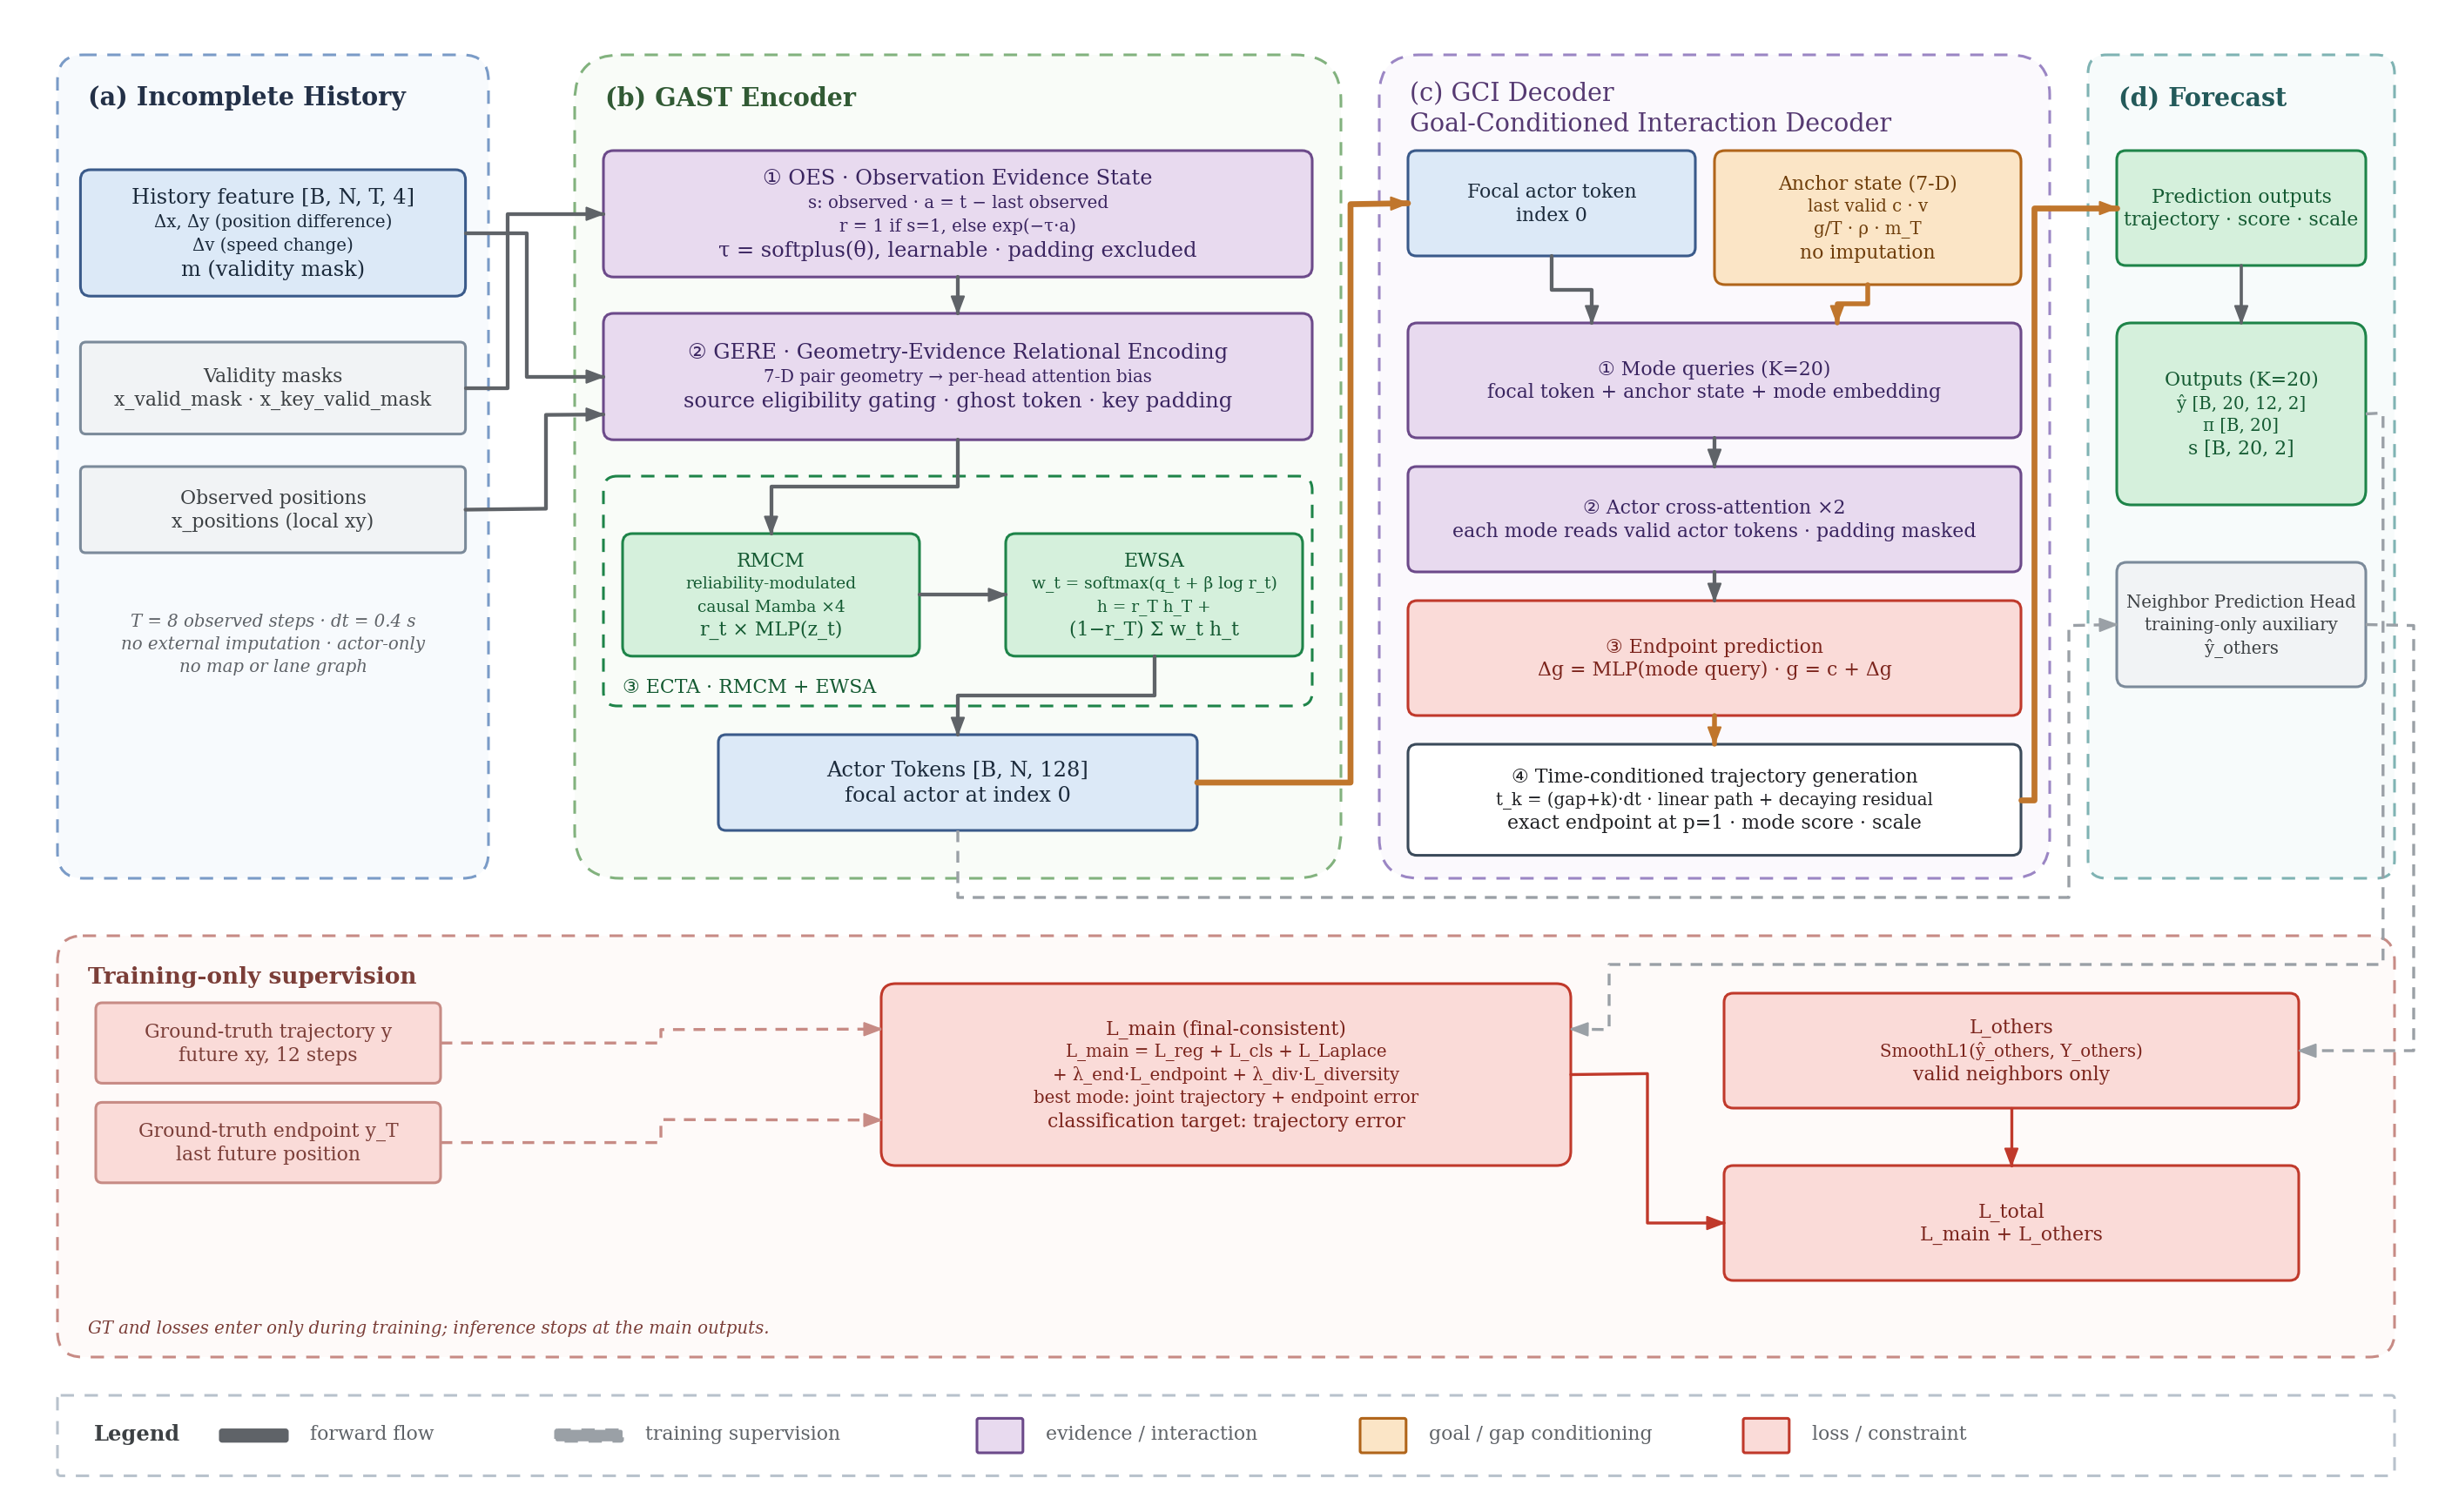
\includegraphics[width=0.94\textwidth]{figures/architecture_crop.png}
\caption{GAST 整体结构。(a) 带掩码的历史仅由位置、有效性掩码与观测位置表示，缺失项为占位值；(b) 观测证据状态（OES）驱动 GERE 与 ECTA，前者执行带几何偏置与源资格约束的逐帧关系注意力，后者按证据强度缩放时间输入（RMCM）并以证据加权方式聚合状态（EWSA）；(c) 目标条件化解码器由最后观测帧构造七维锚点状态（Anchor State），形成 $K$ 个模式查询，并为每个模式预测终点与随进度衰减的残差；(d) 输出 $K$ 条带概率与逐模式尺度的轨迹，邻居预测头仅在训练阶段使用。}
\label{fig:arch}
\end{figure*}

\subsection{观测证据状态}
\label{sec:oes}

对行人 $i$ 与历史步 $t$，记
\begin{equation}
a_{i,t}=t-\max\{t'\le t: m_{i,t'}=1\},
\label{eq:age}
\end{equation}
为距最近一次观测的年龄；当 $t$ 之前不存在有效观测时取 $a_{i,t}=t$（相当于假定窗口之前存在一次虚拟观测）。该状态包含三个量：资格 $s_{i,t}=m_{i,t}$，用于判定该帧能否作为证据来源；年龄 $a_{i,t}$；以及可靠度
\begin{equation}
r_{i,t}=m_{i,t}+(1-m_{i,t})\,\exp(-\tau\,a_{i,t}),\quad \tau=\mathrm{softplus}(\vartheta),
\label{eq:reliability}
\end{equation}
其中 $\vartheta$ 为单一可学习标量，初始化使其满足 $\tau\approx0.1$。可靠度在观测帧上恰为 1，在缺口内单调衰减。填充行的状态被排除，其 $r$ 置零。

式~\eqref{eq:reliability} 有两个性质值得强调。第一，它不是标定后的概率，本文也从不将其解释为概率：它是任务内部的可靠度变量，作用是按证据支持度为历史状态排序。第二，它在完整历史上为恒等映射（$r\equiv1$），此时证据条件化消失，GAST 退化为其骨干网络。这使本文模型能够在无分布偏移的前提下与完整历史结构进行比较。

\subsection{GERE：带几何偏置的逐帧关系编码}
\label{sec:gere}

行人 $i$ 在每一帧的输入为四维向量
\begin{equation}
u_{i,t}=\big[\Delta p_{i,t},\ \Delta s_{i,t},\ m_{i,t}\big],
\label{eq:input}
\end{equation}
分别对应位置增量、观测速度增量与有效性标记，经 patch 嵌入得到 $h_{i,t}=\mathrm{PatchEmbed}(u_{i,t})$。

\textbf{幽灵标记。}每一帧把整个场景的有效性模式池化为一个标记：
\begin{equation}
g_{t}=\mathrm{max}_{i\in\mathcal{V}_{t}}\ \psi\big(\mathbf{1}-m_{i,t}\big),
\label{eq:ghost}
\end{equation}
其中 $\psi$ 为作用于“标量掩码在通道维广播后”的两层嵌入，$\mathcal{V}_{t}$ 为非填充行人的集合。该标记沿用文献 \cite{xu2025sportstraj} 的逐帧空间编码设计，并将其适配到带掩码的历史。标记被前置到该帧的 $N$ 个行人标记之前参与注意力，计算后移除。由于其输入仅为掩码，幽灵标记概括了“当前谁可被观测”，不携带任何位置内容，因而不会注入虚假坐标；但它为所有行人提供了关于场景当前可观测性的共享描述。

\textbf{源资格。}注意力的键只允许取自幽灵标记与满足 $s_{j,t}=1$ 的行人；所有行人（包括未被观测者）仍是合法的查询。因此未被观测的行人可以读取邻居与场景摘要的当前状态，而其自身的陈旧特征不会被其他行人关注。这实现了 P2，也与“仅把掩码作为特征拼接”不同——后者会把陈旧标记留在键集合中。

\textbf{几何偏置。}对每个有序对 $(i,j)$，模型由观测几何构造七维关系描述子
\begin{equation}
f_{ij,t}=\big[\Delta p_{ij},\log(1+\|\Delta p_{ij}\|),\Delta v_{ij},\cos\Delta\theta_{ij},\sin\Delta\theta_{ij}\big],
\label{eq:geom}
\end{equation}
其中 $\Delta p_{ij}=p_{j,t}-p_{i,t}$，$\Delta v_{ij}=v_{j,t}-v_{i,t}$，$\Delta\theta_{ij}$ 为朝向角之差。速度由当前观测位置与前一\emph{有效}位置之差除以两者间的步数估计，因此缺口不会造成速度尖峰；若对中任一端未被观测，则 $f_{ij,t}=\mathbf{0}$。该描述子被映射为每个注意力头一个偏置，
\begin{equation}
B_{ij,t}^{(h)}=w_{2}^{(h)\top}\,\mathrm{GELU}\big(W_{1}f_{ij,t}\big),
\label{eq:bias}
\end{equation}
并加到行人—行人注意力块的 logits 上。式~\eqref{eq:bias} 的输出投影零初始化，因此训练从“无几何”的关系编码器出发，只有在该偏置确实降低目标函数时才被学习。关系编码逐帧进行，输出为每个行人的空间状态序列。

\subsection{ECTA：证据条件化因果时间聚合}
\label{sec:ecta}

\textbf{RMCM（可靠度调制的因果编码器）。}空间状态先经投影，再按可靠度缩放后进入因果递推：
\begin{equation}
\tilde{x}_{i,t}=\mathrm{MLP}(x_{i,t})\cdot r_{i,t},
\qquad
u_{i,1:T}=\mathrm{SSM}_{\phi}(\tilde{x}_{i,1:T}),
\label{eq:rmcm}
\end{equation}
其中 $\mathrm{SSM}_{\phi}$ 为四层单向选择性状态空间块 \cite{gu2023mamba}。因果性是必需的：预测不得依赖未来的历史位置，同时也使编码器可用于流式部署。调制是逐帧、通道共享的标量，改变的是状态进入递推的强度而非状态本身的含义。具体而言，观测帧以单位强度进入，而连续缺失三步的帧被 $e^{-3\tau}$ 衰减，从而难以用衰减后的状态覆盖最后一次可靠状态。

\textbf{EWSA（证据加权状态聚合）。}读出不再固定取最后一个时间步。以内容得分 $e_{i,t}=w^{\top}u_{i,t}$、温度 $\beta=1$，模型计算
\begin{equation}
\alpha_{i,t}=\mathrm{softmax}_{t}\big(e_{i,t}+\beta\log r_{i,t}\big),\qquad
\bar{h}_{i}=\sum_{t}\alpha_{i,t}\,u_{i,t},
\label{eq:ewsa}
\end{equation}
并以末端可靠度在末端状态与该聚合之间做门控：
\begin{equation}
z_{i}=r_{i,T}\,u_{i,T}+\big(1-r_{i,T}\big)\bar{h}_{i}.
\label{eq:gate}
\end{equation}
当末帧被观测时 $z_{i}=u_{i,T}$，读出与标准的末端读出完全一致；当末帧缺失时，模型回退到可用状态的加权平均，权重同时受学习到的内容得分与证据强度塑形。该门控在形式上是硬切换，在数值上是软过渡，因为 $r_{i,T}$ 随末端缺口连续衰减。

\subsection{锚点条件化目标解码}
\label{sec:decoder}

\textbf{锚点状态（Anchor State）。}设 $\ell_{i}$ 为最后一个有效观测帧的下标，$\ell'_{i}$ 为其前一个有效观测帧的下标。解码器接收
\begin{equation}
\varphi_{i}=\Big[p_{i,\ell_i},\ v_{i},\ \tfrac{\delta_{i}}{T},\ \rho_{i},\ \mathbb{1}[\ell_{i}<T]\Big]\in\mathbb{R}^{7},
\label{eq:anchor}
\end{equation}
其中 $\delta_{i}=T-\ell_{i}+1$ 为末次观测到预测起点的步数，$v_{i}=(p_{i,\ell_i}-p_{i,\ell'_i})/(\ell_i-\ell'_i)$ 为缺口感知速度（只有一帧观测时为零），$\rho_{i}=\frac{1}{T}\sum_{t}m_{i,t}$ 为有效观测比例，末项标记末端缺失。保留锚点位置分量是为使该模块在任意坐标系下有定义；在第~\ref{sec:task} 节的锚点中心化归一化下该分量恒为零，状态信息由速度与间隔描述子承载。

\textbf{模式查询。}由式~\eqref{eq:gate} 得到的行人表示 $z_{i}$ 与锚点嵌入 $e^{\varphi}_{i}=\mathrm{MLP}(\varphi_{i})$ 同可学习的逐模式嵌入 $e_{k}$ 相加，
\begin{equation}
q_{i,k}=z_{i}+e^{\varphi}_{i}+e_{k},\qquad k=1,\dots,K,
\label{eq:query}
\end{equation}
再由两层交叉注意力在场景的行人表示上细化，填充行被屏蔽。每个模式因此在其自身的锚点条件下读取上下文，而不是共享单一场景向量。

\textbf{终点与轨迹。}一个预测头把每个模式查询映射为相对锚点的位移，
\begin{equation}
\hat{y}_{i,k,H}=p_{i,\ell_i}+\Delta_{i,k},\qquad \Delta_{i,k}=\mathrm{MLP}(q_{i,k}).
\label{eq:endpoint}
\end{equation}
对第 $t=1,\dots,H$ 步，令 $\tau_{t}=\delta_{i}+t-1$ 为锚点时刻到该未来步的经过步数，$p_{t}=\tau_{t}/(\delta_{i}+H-1)$ 为锚点—终点区间上的相对进度。轨迹由直线骨架与衰减残差构成：
\begin{equation}
\hat{y}_{i,k,t}=p_{i,\ell_i}+p_{t}\Delta_{i,k}+(1-p_{t})\,g_{\psi}(q_{i,k},e(\Delta_{i,k}),e(\tau_{t}\Delta t)).
\label{eq:traj}
\end{equation}
该构造有三点后果。第一，首个预测点已沿骨架推进 $\delta_{i}/(\delta_{i}+H-1)$，因此较长的末端缺口不会被默认为“行人停留在最后观测位置”。第二，残差在预测初期拥有完整自由度，且在 $t=H$ 处严格为零，使输出终点与预测目标一致。第三，由于 $p_{t}$ 以实际间隔为单位定义，同一模块无需特例即可处理观测末帧与末端缺失样本。

\textbf{模式概率与尺度。}评分头读取模式查询、终点嵌入与逐步查询的均值，输出 logits，经 softmax 得到 $\pi_{i,k}$。另一并行的头输出逐步、逐轴的 Laplace 尺度 $\sigma_{i,k,t}=\mathrm{ELU}(\cdot)+1.0001$，供下文似然项使用；$\sigma$ 是预测分布的离散度参数，不是标定后的置信区间。

\subsection{训练目标}
\label{sec:loss}

监督施加于目标行人（每个场景样本的第 0 个位置）。对模式 $k$，计算平均位移 $d_{k}$ 与终点误差 $d^{\mathrm{end}}_{k}$，并定义联合误差 $J_{k}=d_{k}+\lambda_{e}d^{\mathrm{end}}_{k}$，取 $\lambda_{e}=1$。两个不同的模式被用于两个不同目的：回归模式 $k^{\ast}=\arg\min_{k}J_{k}$ 兼顾形状与目的地，分类目标 $k^{\dagger}=\arg\min_{k}d_{k}$ 仅由轨迹级误差定义。总损失为
\begin{equation}
\mathcal{L}=\mathcal{L}_{\mathrm{reg}}+\mathcal{L}_{\mathrm{cls}}
+\mathcal{L}_{\mathrm{NLL}}+\mathcal{L}_{\mathrm{end}}
+\lambda_{d}\mathcal{L}_{\mathrm{div}}+\mathcal{L}_{\mathrm{nbr}},
\label{eq:loss}
\end{equation}
其中 $\mathcal{L}_{\mathrm{reg}}=\mathrm{SmoothL1}(\hat{y}_{k^{\ast}},y)$，$\mathcal{L}_{\mathrm{cls}}=-\log\pi_{k^{\dagger}}$，$\mathcal{L}_{\mathrm{end}}=\mathrm{SmoothL1}(\hat{y}_{k^{\ast},H},y_{H})$，$\mathcal{L}_{\mathrm{nbr}}=\mathrm{SmoothL1}(\hat{y}^{\mathrm{nbr}},y^{\mathrm{nbr}})$，$\mathcal{L}_{\mathrm{div}}=\mathbb{E}_{k\ne l}[0.5-\|\hat{y}_{k,H}-\hat{y}_{l,H}\|]_{+}$ 为终点两两距离上的合页项；$\mathcal{L}_{\mathrm{NLL}}$ 为附录~\ref{app:loss} 详述的 Laplace 负对数似然。交叉熵使用标签平滑 $0.2$，多样性权重 $\lambda_{d}=0.05$，间隔为 $0.5$~m。似然项在轨迹最接近的模式上计算，形式为逐步、逐轴平均的 $\log(2\sigma)+|y-\hat{y}|/\sigma$，并与软目标交叉熵 $0.5\sum_{k}\tilde{\pi}_{k}\log\pi_{k}$ 组合，其中 $\tilde{\pi}$ 由负轨迹误差经温度 softmax 得到；该项用于标定离散度并柔和地塑造模式分布，而不与硬分类目标竞争。邻居项由其他行人的编码状态预测其未来，仅在训练阶段生效；推理阶段模型只返回目标行人的 $K$ 条候选轨迹及其概率。

将 $k^{\ast}$ 与 $k^{\dagger}$ 分离是有意为之。概率应当按“模式对整条轨迹的解释程度”排序，而终点头应当在最符合目的地的模式上训练。若共用同一指派，必有一个目标被迫让步；分离二者在推理阶段不带来任何额外代价。

\subsection{性质}

\textbf{精确退化。}当所有 $m_{i,t}=1$ 时，式~\eqref{eq:reliability} 给出 $r\equiv1$：式~\eqref{eq:rmcm} 退化为普通因果编码器，式~\eqref{eq:gate} 返回末端状态，锚点状态仅承载观测速度，且 $\delta=1$、$\rho=1$、无末端缺失标记。此时缺失专用机制不产生任何作用，与完整历史基线之间的差异可归因于解码器与始终存在的场景级标记。

\textbf{无信息泄漏。}占位值不会进入任何差分、距离或速度计算：速度只在观测帧之间计算，成对几何在任一端未被观测时置零，未被观测的行人被移出键集合；真值未来仅在损失中使用。

\textbf{计算代价。}模型共 1.19M 参数（编码器 0.60M，解码器 0.55M），推理为一次前向，$K=20$ 个模式查询并行完成，无需采样循环。逐帧关系注意力的复杂度为帧内行人数 $N$ 的 $O(N^{2})$，与本文对比的社会注意力基线同阶。

\section{实验}
\label{sec:exp}

\subsection{实验设置}
\label{sec:setup}

\textbf{数据与协议。}全部实验采用第~\ref{sec:bench} 节的 TrajGap-Bench Mixed 协议：Mixed-train 用于拟合，Mixed-val 用于按最终预测头的 $\mathrm{minFDE}_{20}$ 选择检查点，Mixed-test 仅评估一次；五个场景，$T=8$，$H=12$，$K=20$。依照数据发布的逐场景划分，每个场景训练一个模型。所有方法均在自然的 Mixed 分布上训练，不按缺失帧数重新加权。

\textbf{实现细节。}GAST 的嵌入宽度为 128，注意力头数为 8，时间栈包含四层选择性状态空间块，解码器含两层交叉注意力，$K=20$，dropout 与 drop-path 均为 0.2。训练使用 AdamW，学习率 $10^{-3}$，权重衰减 $10^{-4}$，预热 5 个轮次，梯度裁剪范数 5，批大小 64，bf16 混合精度，最多 100 个轮次；实际选中的检查点位于第 33 至 58 轮之间，故训练预算不构成约束。每个场景使用单张 NVIDIA RTX 5880 Ada GPU 训练。模型参数量为 1.19M。所有方法的随机种子固定为 2024。

\textbf{对比方法。}本文与六种外部方法对比，覆盖两类。
\begin{itemize}
\item \emph{完整历史预测器。}\textbf{SocialLSTM} \cite{alahi2016social} 采用缺失感知变体（零占位、缺失帧跳过 LSTM 状态更新、$K=20$ 的高斯混合头）。\textbf{AgentFormer} \cite{yuan2021agentformer} 接收逐帧有效性通道，并以最后观测帧作为解码锚点。\textbf{MoFlow} \cite{fu2025moflow} 使用官方实现，配以掩码感知特征，缺失步以逐通道均值占位。\textbf{Re} \cite{mao2025resonance} 以零填充历史原样运行。
\item \emph{插补感知与图结构预测器。}\textbf{MS-TIP} \cite{chib2024mstip} 将基于 SAITS 的插补分支与预测器耦合、端到端训练，代表直接输入约束下的“插补—预测”路线。\textbf{Social-STGCNN} \cite{mohamed2020social} 作为图结构参照，缺失行人被表示为既不发送也不接收消息的幽灵节点。
\end{itemize}
不具备模式概率头的方法（AgentFormer、Re、MS-TIP、Social-STGCNN）不参与 top-1 诊断，但参与仅需 $K$ 条候选的主指标。所有方法读取完全相同的测试张量。

\subsection{主要结果}
\label{sec:main}

表~\ref{tab:main} 给出主对比结果。GAST 在两项指标上均取得最优宏平均（0.3168/0.4831~m）与最优微平均（0.2894/0.4716~m）。相对最强外部基线（MoFlow），宏平均上 $\mathrm{minADE}_{20}$ 降低 9.4\%、$\mathrm{minFDE}_{20}$ 降低 7.6\%，微平均上降低 7.5\%/5.3\%。GAST 在 $\mathrm{minADE}_{20}$ 上对 MoFlow 五个场景全胜，在 $\mathrm{minFDE}_{20}$ 上四胜一负，唯一例外是 ZARA1-M，MoFlow 在该场景优 1.8\%。

逐场景结果比聚合值更能说明问题。GAST 在 ETH-M、UNIV-M、ZARA1-M 与 ZARA2-M 上取得最优 $\mathrm{minADE}_{20}$，在 ETH-M、UNIV-M 与 ZARA2-M 上取得最优 $\mathrm{minFDE}_{20}$。在 HOTEL-M 上 AgentFormer 明显更优（0.2083/0.3316 对 0.2541/0.3769），在 ZARA1-M 的 $\mathrm{minFDE}_{20}$ 上 MoFlow 略优（0.4057 对 0.4128）。可见 GAST 的优势并不覆盖所有场景，其宏平均领先来自 ETH-M 与 UNIV-M 上较大幅度的收益；第~\ref{sec:disc} 节讨论何种场景特征与方法收益相关。

两种最弱的基线差距明显。MS-TIP 作为插补感知联合训练的代表位列倒数第二，以幽灵节点表示缺失行人的 Social-STGCNN 位列末位。二者与其他方法遵循同一评测契约，因此差距并非协议造成；它反映的是 8 帧历史、最多缺失七帧且缺口频繁延伸至预测起点这一设定的难度。经典社会池化模型同样明显落后（0.4576/0.6079），考虑到历史很短且其缺失感知变体缺乏显式多模态建模，这一结果在预期之内。

\begin{table*}[t]
\centering
\scriptsize
\setlength{\tabcolsep}{2.4pt}
\caption{TrajGap-Bench Mixed-test 主结果（$K=20$，随机种子 2024）。单元格为 $\mathrm{minADE}_{20}$/$\mathrm{minFDE}_{20}$，单位米，越低越好。Macro 为五场景宏平均，Micro 为按测试样本数加权的微平均。逐场景、逐指标最优加粗。标 $\dagger$ 的方法输出无权重样本，不参与 top-1 诊断。}
\label{tab:main}
\begin{tabular}{@{}lccccccc@{}}
\toprule
Method & ETH-M & HOTEL-M & UNIV-M & ZARA1-M & ZARA2-M & Macro & Micro \\
\midrule
\textbf{GAST (ours)} & \textbf{0.5852}/\textbf{0.8212} & 0.2541/0.3769 & \textbf{0.3200}/\textbf{0.5244} & \textbf{0.2510}/0.4128 & \textbf{0.1738}/\textbf{0.2801} & \textbf{0.3168}/\textbf{0.4831} & \textbf{0.2894}/\textbf{0.4716} \\
MoFlow & 0.6819/0.9389 & 0.2777/0.4247 & 0.3478/0.5572 & 0.2566/\textbf{0.4057} & 0.1839/0.2867 & 0.3496/0.5227 & 0.3129/0.4981 \\
AgentFormer & 0.7098/1.0436 & \textbf{0.2083}/\textbf{0.3316} & 0.4132/0.6796 & 0.3551/0.5795 & 0.2690/0.4375 & 0.3911/0.6144 & 0.3795/0.6220 \\
SocialLSTM & 0.8430/1.0456 & 0.2924/0.3871 & 0.4543/0.6512 & 0.4126/0.5650 & 0.2858/0.3907 & 0.4576/0.6079 & 0.4193/0.5941 \\
Re$^{\dagger}$ & 0.9945/1.4262 & 0.7799/1.2808 & 0.5388/0.8408 & 0.4960/0.7470 & 0.3819/0.5928 & 0.6382/0.9775 & 0.5187/0.8085 \\
MS-TIP$^{\dagger}$ & 1.6345/2.0985 & 1.3102/1.5472 & 1.3240/1.1566 & 0.8842/1.1720 & 0.7663/0.9902 & 1.1838/1.3929 & 1.1991/1.1461 \\
Social-STGCNN$^{\dagger}$ & 2.1393/3.5048 & 1.3022/2.1624 & 0.9496/1.5336 & 1.4801/2.7038 & 0.8646/1.5258 & 1.3471/2.2861 & 0.9878/1.6409 \\
\bottomrule
\end{tabular}
\end{table*}

\subsection{缺失程度增加下的行为}
\label{sec:severity}

表~\ref{tab:severity} 与图~\ref{fig:degrad} 按历史缺失帧数对测试集分层。基准的官方扫描使缺失 $0$ 至 $7$ 帧的每个桶在测试集上等权（每桶 33{,}654 个样本；缺失四帧的桶为 67{,}308，因为 ETH-M 在该桶贡献了两份），因此各桶可直接比较。

各曲线在聚合值之外给出更清晰的分离。GAST 在缺失零至六帧区间退化最平缓：$\mathrm{minFDE}_{20}$ 由 0.3592 升至 0.4281~m（$+19\%$），而 MoFlow 由 0.3793 升至 0.5534~m（$+46\%$）。相对 MoFlow 的优势并非常数，而是随严重程度扩大：缺失零帧时 $-5.4\%$，三帧时 $-11.2\%$，五帧时 $-14.8\%$，六帧时 $-22.6\%$；$\mathrm{minADE}_{20}$ 上对应的变化为 $-6.7\%$ 至 $-25.9\%$。这一“剂量—效应”形态与证据条件化的设计意图一致，即收益应随可用证据减少而增大。

缺失七帧时仅剩一个观测。此时排序发生反转：MoFlow 的 $\mathrm{minFDE}_{20}$ 为 1.2224~m，优于 GAST 的 1.2731~m（$+4.1\%$）；$\mathrm{minADE}_{20}$ 上 MoFlow 亦更优（0.8734 对 0.9126）。只有一帧时不存在可利用的速度、朝向与缺口结构，预测由学习到的先验决定，为证据路由而正则化的模型已无证据可路由。本文将其视为该区间的边界而非模型失效，但这确实意味着不应宣称 GAST 改善了单帧情形。

\begin{table*}[t]
\centering
\footnotesize
\setlength{\tabcolsep}{4.6pt}
\caption{按历史缺失帧数分层的结果（五场景宏平均，单位米）。除缺失四帧为 67{,}308 个样本外，其余各桶均为 33{,}654 个样本。各桶最优值加粗。}
\label{tab:severity}
\begin{tabular}{@{}lcccccccc@{}}
\toprule
 & 0 & 1 & 2 & 3 & 4 & 5 & 6 & 7 \\
\midrule
\multicolumn{9}{@{}l}{\emph{$\mathrm{minADE}_{20}$}}\\
GAST & \textbf{0.2154} & \textbf{0.2192} & \textbf{0.2286} & \textbf{0.2336} & \textbf{0.2440} & \textbf{0.2629} & \textbf{0.2911} & 0.9126 \\
MoFlow & 0.2309 & 0.2390 & 0.2481 & 0.2706 & 0.2847 & 0.3221 & 0.3926 & \textbf{0.8734} \\
\midrule
\multicolumn{9}{@{}l}{\emph{$\mathrm{minFDE}_{20}$}}\\
GAST & \textbf{0.3590} & \textbf{0.3632} & \textbf{0.3756} & \textbf{0.3777} & \textbf{0.3854} & \textbf{0.4002} & \textbf{0.4281} & 1.2731 \\
MoFlow & 0.3793 & 0.3889 & 0.3968 & 0.4254 & 0.4341 & 0.4695 & 0.5534 & \textbf{1.2224} \\
\bottomrule
\end{tabular}
\end{table*}

\begin{figure*}[t]
\centering
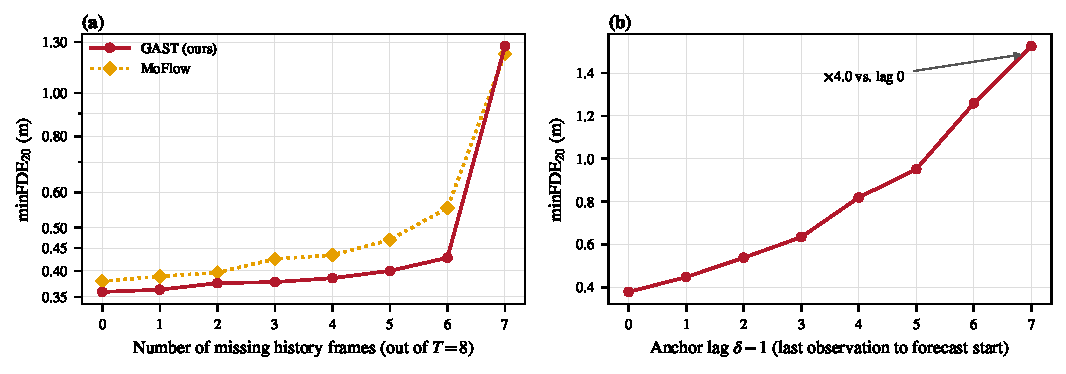
\includegraphics[width=\textwidth]{figures/degradation_en.pdf}
\caption{退化与证据损失（五场景宏平均）。(a) $\mathrm{minFDE}_{20}$ 随历史缺失帧数的变化，纵轴为对数刻度；缺失七帧处反映仅剩一次观测的区间变化。(b) $\mathrm{minFDE}_{20}$ 随锚点间隔（末次观测到预测起点的步数）的变化，间隔 7 处的误差约为间隔 0 的 4.0 倍。}
\label{fig:degrad}
\end{figure*}

\subsection{末端缺失与锚点间隔}
\label{sec:lag}

表~\ref{tab:lag} 沿两个被缺失计数混淆的轴描述 GAST 的误差结构。末端缺失把缺口延伸至预测起点的样本与缺口提前结束的样本分开，锚点间隔则计数末次观测到起点的步数。由于公开基线未提供相同粒度的分层预测，本节仅报告 GAST 自身的分层结果，用于刻画误差随证据年龄的增长方式。

误差随锚点间隔单调上升：$\mathrm{minFDE}_{20}$ 从间隔 0 的 0.3787~m 增至间隔 7 的 1.5260~m，约为前者的 4.0 倍；$\mathrm{minADE}_{20}$ 由 0.2272~m 增至 1.1847~m。增长并非线性：间隔 0 至 2 每增加一步约抬升 18\%–42\%，间隔 3 之后每步抬升幅度更大，至间隔 7 达到 303\%。这表明当末次观测远离预测起点时，误差主要由锚点状态的陈旧程度决定，而非由场景差异决定。

末端缺失组的 $\mathrm{minFDE}_{20}$ 为 0.6112~m，比非末端组的 0.3787~m 高 61.4\%；$\mathrm{minADE}_{20}$ 相应高 87.9\%。这正是锚点状态与进度参数化骨架所针对的条件：缺口延伸至起点时，首个预测点必须从陈旧的锚点出发，且其后的未观测区间完全不可见。间隔 7 处的极端值提示可靠度衰减应在某一年龄之后饱和，而不是持续偏好极旧的状态；本文将这一点作为当前形式的局限而非调优结果。

\begin{table}[t]
\centering
\footnotesize
\setlength{\tabcolsep}{3.4pt}
\caption{GAST 按锚点间隔与末端缺失分层的结果（五场景宏平均）。单元格为 $\mathrm{minADE}_{20}$/$\mathrm{minFDE}_{20}$，单位米；$\Delta$ 为相对锚点间隔 0 的 $\mathrm{minFDE}_{20}$ 变化，非末端组与间隔 0 为同一批样本。}
\label{tab:lag}
\begin{tabular}{@{}l c c r@{}}
\toprule
Group & $n$ & GAST & $\Delta$FDE \\
\midrule
lag 0 & 167{,}469 & 0.2272/0.3787 & --- \\
lag 1 & 60{,}284 & 0.2887/0.4480 & $+18.3\%$ \\
lag 2 & 30{,}263 & 0.3581/0.5384 & $+42.2\%$ \\
lag 3 & 17{,}368 & 0.4477/0.6345 & $+67.6\%$ \\
lag 4 & 10{,}763 & 0.6051/0.8195 & $+116.4\%$ \\
lag 5 & 7{,}379 & 0.7564/0.9515 & $+151.3\%$ \\
lag 6 & 5{,}356 & 0.9577/1.2590 & $+232.5\%$ \\
lag 7 & 4{,}004 & 1.1847/1.5260 & $+303.0\%$ \\
\midrule
terminal & 135{,}417 & 0.4268/0.6112 & $+61.4\%$ \\
\bottomrule
\end{tabular}
\end{table}

\subsection{覆盖度与排序}
\label{sec:coverage}

表~\ref{tab:top1} 报告 top-1 诊断。GAST 的 $\mathrm{ADE@1}$/$\mathrm{FDE@1}$ 为 0.9806/1.7887~m，与 MoFlow 的 0.9814/1.7296~m 基本相当：$\mathrm{ADE@1}$ 略优 0.1\%，$\mathrm{FDE@1}$ 略差 3.4\%；相对 SocialLSTM 则分别优 26.1\% 与 18.2\%。将这一结果与主指标对照可知，GAST 相对 MoFlow 在 best-of-20 上取得的 9.4\%/7.6\% 提升并未同步体现在概率最高的单一模式上。

这一分离对使用方式有直接影响。best-of-20 衡量的是候选集合对真实未来的覆盖能力，而部署在规划器之后的预测器通常只消费概率最高的模式。因此 GAST 的收益更适用于对候选集合做保守规划或集成的场合；若下游仅依赖 top-1，则其相对 MoFlow 的优势将收窄至统计噪声量级。排序质量的改进需要单独设计模式评分目标，本文未对此作进一步处理，并将其列为开放问题。

\begin{table}[t]
\centering
\footnotesize
\setlength{\tabcolsep}{4.2pt}
\caption{top-1 诊断（宏平均，单位米）。$\mathrm{ADE@1}$/$\mathrm{FDE@1}$ 取概率最高的模式。无模式概率的方法未列入。}
\label{tab:top1}
\begin{tabular}{@{}lcc@{}}
\toprule
Method & $\mathrm{ADE@1}$ & $\mathrm{FDE@1}$ \\
\midrule
GAST & \textbf{0.9806} & 1.7887 \\
MoFlow & 0.9814 & \textbf{1.7296} \\
SocialLSTM & 1.3278 & 2.1865 \\
\bottomrule
\end{tabular}
\end{table}

\subsection{可复现性}
\label{sec:repro}

评测协议、Mixed 适配器、训练入口、评估器与模型配置以单一代码仓库发布。每次运行写出 manifest，记录 git 版本、解析后的配置、所消费的数据文件、检查点规则与环境信息（Python、PyTorch 与 CUDA 版本）。评估输出一个 JSON 文件，包含五个分层维度的逐样本诊断；本文全部表格由脚本从这些文件生成，而非手工转抄。Laplace 似然存在两种数值等价的实现，其中一种为向量化版本；等价性门禁校验二者梯度在机器精度内一致，每次运行实际使用的实现记录在其 manifest 中。

\section{讨论}
\label{sec:disc}

\subsection{收益出现的位置}

分层结果支持对该方法的一种特定解读。GAST 的相对优势并非均匀分布，而是随可用证据减少而扩大：相对 MoFlow，历史完整时 $\mathrm{minFDE}_{20}$ 降低 5.4\%，缺失三帧时降低 11.2\%，五帧时降低 14.8\%，六帧时降低 22.6\%；$\mathrm{minADE}_{20}$ 上对应为 6.7\% 至 25.9\%。当仅剩一个观测时该趋势反转，GAST 落后 MoFlow 约 4\%。按照证据条件化的设计意图，收益应集中在缺失较多的条件下，因为此时“哪些帧可信、最后一个状态有多旧”对预测的影响最大；观测完整时证据状态退化为恒等，模型与普通完整历史结构无异。观测到的形态与该预期相符。

误差随证据年龄的增长进一步说明问题来源。锚点间隔从 0 增至 7 时，GAST 的 $\mathrm{minFDE}_{20}$ 增至 4.0 倍；末端缺失组的误差比非末端组高 61.4\%。这两项都不是模型间比较，而是同一模型在不同证据条件下的行为，它们表明误差的主要来源是锚点状态的陈旧程度，而非场景本身。

但必须强调，以上只是与机制一致的证据，而非机制归因。本文未报告组件级消融，因此无法把收益分配给逐帧几何证据编码、可靠度调制的时间聚合与锚点条件化解码中的任何一个；同样无法排除模型容量、训练细节或归纳偏置带来的贡献。严格的归因需要在同一训练协议下逐组件开关的四臂实验，本文将其列为后续工作。

\subsection{场景异质性}

逐场景结果并不一致：GAST 在四个场景上取得最优 $\mathrm{minADE}_{20}$、在三个场景上取得最优 $\mathrm{minFDE}_{20}$，但在 HOTEL-M 上落后 AgentFormer（0.2541/0.3769 对 0.2083/0.3316），在 ZARA1-M 的 $\mathrm{minFDE}_{20}$ 上落后 MoFlow（0.4128 对 0.4057）。本文可以给出一个假设，尽管该基准无法对其进行干净的检验。HOTEL-M 与 ZARA1-M 的运动较慢、较规则，且受场景约束较强，从最后观测出发的单模态外推已经足够准确；以在多个不同目的地上分配概率质量为目标的目标条件化解码器，在此类场景中增加方差而不增加精度。ETH-M 与 UNIV-M 的运动更异质、方向变化更频繁，目的地本身更不确定，显式的终点假设因而有帮助。若该解读成立，解码器应依据场景级或样本级的终点不确定性估计进行条件化，而不是统一施加。本文认为这是缩小场景差距最有希望的方向，但当前证据只是相关性。

\subsection{覆盖度与排序}

best-of-20 覆盖度与 top-1 排序之间的落差是本研究中值得注意的现象。GAST 在 best-of-20 上相对 MoFlow 降低 9.4\%/7.6\%，但在概率最高的单一模式上两者基本相当（$\mathrm{ADE@1}$ 优 0.1\%，$\mathrm{FDE@1}$ 差 3.4\%）。换言之，收益主要来自候选集合对真实未来的覆盖能力提升，而非模式评分对最优候选的识别能力提升。

这一落差对使用方式有直接影响。best-of-20 适用于对候选集合做保守规划或集成的场合；若下游规划器只消费 top-1，本方法的优势将收窄至噪声量级。要同时改善排序，需要在训练目标中显式优化模式概率与轨迹质量的对应关系，例如引入排序损失或对模式评分做校准，而不是仅依赖轨迹级分类标签。本文未对此作进一步处理，并将其列为开放问题。

\subsection{局限性}

\textbf{单随机种子。}所有数值均来自每个场景的一次运行，没有置信区间。开发过程中同一配置在 UNIV-M 上的两次运行曾相差 4.4\%，因此单场景上几个百分点的差异（例如 ZARA1-M 上 1.8\% 的 $\mathrm{minFDE}_{20}$ 差距）处于噪声范围内。宏平均上 9.4\%/7.6\% 的领先大于该波动，但仍应视为单种子结论；在声称稳定改进之前，需要多种子研究与按轨迹聚类的配对自助重采样。

\textbf{协议依赖。}TrajGap-Bench 是基于合成掩码的受控压力测试，其缺失分布不对应任何真实跟踪器，且基准限定于五个 ETH/UCY 场景与 8 帧历史。真实感知输出与其他数据集（如 SDD 或 Argoverse）上的外部效度尚未验证。

\textbf{测试集依赖性。}测试划分中包含同一潜在轨迹在多个掩码下的多次出现。本文的聚合把样本视为独立，这会高估任何显著性陈述的有效样本量。发布的逐样本诊断包含源轨迹标识，正是为了便于后续进行聚类推断。

\textbf{缺少组件级消融。}本文报告的是完整模型与外部基线的对比，未逐一移除逐帧几何证据编码、可靠度调制的时间聚合与锚点条件化解码。因此方法内部的贡献分配尚不清楚，也无法判断某一模块是否可以被更简单的结构替代。

\textbf{缺失的对比。}本文未在直接预测表中报告两阶段插补基线，因为该设置向模型暴露更多信息、必须单独报告；因此这是对比的缺失，而非阴性结果。本文亦未报告推理时延，而这对部署是重要的。

\subsection{对基准设计的启示}

协议中有两项设计被证明是承重的。将 Easy 与 Hard 合并为单一 Mixed 划分，使模型无法在“自己恰好最强的难度”上被选中，并使缺失计数分层成为诊断而非榜单。把检查点固定为最终预测头的验证集 $\mathrm{minFDE}_{20}$，消除了一个原本会因论文而异的自由度。两项选择都易于采纳，且据本文经验会改变结论：在按难度分别选点的口径下，不同检查点之间的排序可以发生改变，因而跨论文比较必须依赖统一的选点规则。本文建议后续缺失历史预测工作报告至少缺失帧数与末端缺失两项分层，因为聚合值可能掩盖文中七帧处记录的反转。

\section{结论}
\label{sec:concl}

本文主张，不完整历史应被视为一种预测条件，而非有待修复的数据，并以一个协议与一个模型支撑该主张。TrajGap-Bench 在公开 TrajImpute 发布上冻结单一 Mixed 契约——一种划分构造、一条检查点规则、两项指标、五个诊断分层——使所有消费不完整历史的方法可以在相同条件下比较。GAST 使观测证据状态贯穿逐帧关系注意力、可靠度调制的因果状态空间编码器与锚点条件化目标解码器，且从不对坐标做插补。

在五个场景共 302{,}886 个测试样本上，GAST 取得对比方法中最优的宏平均 best-of-20 误差（0.3168/0.4831~m），相对最强外部基线 MoFlow 降低 9.4\%/7.6\%，并在 $\mathrm{minADE}_{20}$ 上对 MoFlow 五个场景全胜、在 $\mathrm{minFDE}_{20}$ 上四胜一负。该优势与证据条件化的设计意图一致：相对 MoFlow 的 $\mathrm{minFDE}_{20}$ 降低幅度由无缺失时的 5.4\% 增至缺失六帧时的 22.6\%，并在仅剩一个观测时反转。本文同时报告了两项限定该贡献的结果：改进并不跨场景一致（HOTEL-M 与 ZARA1-M 的 $\mathrm{minFDE}_{20}$ 分别落后于 AgentFormer 与 MoFlow），且 best-of-20 的提升未同步体现在概率最高的单一模式上。

下一步工作直接来自上述局限。需要多种子研究与按轨迹聚类的统计，以确定相对外部基线的边际是否稳定；需要同一协议下逐组件开关的消融，以分离逐帧几何证据编码、可靠度调制时间聚合与锚点条件化解码的贡献；需要为证据年龄引入饱和规则以处理最旧锚点处的反转；并需要改进模式评分目标，使覆盖度收益能够传递到 top-1。上述协议亦应扩展到其他观测几何与真实感知流程产出的轨迹，后者的缺失分布并非合成。


\appendix
\section{目标函数与实现细节}
\label{app:impl}

\subsection{辅助项的显式形式}
\label{app:loss}

记 $y\in\mathbb{R}^{H\times2}$ 为目标行人的未来，$\hat{y}_{k}$ 为第 $k$ 条候选，$\pi\in\Delta^{K-1}$ 为模式分布。以逐步误差 $e_{k,t}=\|\hat{y}_{k,t}-y_{t}\|$、$d_{k}=\frac{1}{H}\sum_{t}e_{k,t}$、$d^{\mathrm{end}}_{k}=\|\hat{y}_{k,H}-y_{H}\|$，式~\eqref{eq:loss} 中未在正文展开的项为
\begin{equation}
\begin{aligned}
\mathcal{L}_{\mathrm{NLL}}=\ &\frac{1}{2H}\sum_{t,c}\Big[\log\big(2\sigma_{k^{\ast},t,c}\big)+\frac{|y_{t,c}-\hat{y}_{k^{\ast},t,c}|}{\sigma_{k^{\ast},t,c}}\Big]\\
&-\frac{1}{2}\sum_{k}\tilde{\pi}_{k}\log\pi_{k},
\end{aligned}
\label{eq:nll}
\end{equation}
软目标为
\begin{equation}
\tilde{\pi}_{k}=\mathrm{softmax}_{k}(-d_{k}/H),\quad
k^{\ast}=\arg\min_{k}(d_{k}+\lambda_{e}d^{\mathrm{end}}_{k}),
\label{eq:softtarget}
\end{equation}
$\lambda_{e}=1$，$k^{\dagger}=\arg\min_{k}d_{k}$。软目标不回传梯度。分类项 $\mathcal{L}_{\mathrm{cls}}=-\log\pi_{k^{\dagger}}$ 使用标签平滑 $0.2$；多样性项取 $\lambda_{d}=0.05$、间隔 $0.5$~m。邻居项对其余全部非填充行人的未来施加 SmoothL1 损失，由作用于其编码状态的两层预测头给出，仅在训练阶段生效。

\subsection{逐场景分层结果}
\label{app:strat}

表~\ref{tab:appstrat} 给出 GAST 在各场景、各缺失帧数下的 $\mathrm{minFDE}_{20}$。场景层面的形态与宏平均曲线一致：在缺失不超过六帧时 ETH-M 与 HOTEL-M 最不敏感，UNIV-M 与 ZARA1-M 退化更平稳，所有场景在缺失七帧处均出现不连续。HOTEL-M 是最极端的情形：缺失零至六帧时曲线近乎平坦（0.1835 至 0.1957~m），随后跃升至 1.9085~m；这与该场景低速、受强约束的运动特征一致——即使只剩一次观测，也仍能在相当程度上约束目的地。

\begin{table}[t]
\centering
\scriptsize
\setlength{\tabcolsep}{1.0pt}
\caption{GAST 在各场景、各历史缺失帧数下的 $\mathrm{minFDE}_{20}$（单位米）。ETH-M 在缺失四帧的桶中有 362 个样本，其余桶各 181 个；其他场景每个桶各 181 个。}
\label{tab:appstrat}
\begin{tabular}{@{}lcccccccc@{}}
\toprule
Scene & 0 & 1 & 2 & 3 & 4 & 5 & 6 & 7 \\
\midrule
ETH-M   & 0.6641 & 0.6755 & 0.7196 & 0.7001 & 0.6988 & 0.7026 & 0.7314 & 1.7995 \\
HOTEL-M & 0.1835 & 0.1841 & 0.1806 & 0.1841 & 0.1847 & 0.1865 & 0.1957 & 1.9085 \\
UNIV-M  & 0.3997 & 0.4068 & 0.4176 & 0.4270 & 0.4427 & 0.4688 & 0.5048 & 1.2093 \\
ZARA1-M & 0.3199 & 0.3214 & 0.3292 & 0.3392 & 0.3523 & 0.3812 & 0.4185 & 0.9013 \\
ZARA2-M & 0.2276 & 0.2281 & 0.2312 & 0.2379 & 0.2483 & 0.2621 & 0.2902 & 0.5469 \\
\bottomrule
\end{tabular}
\end{table}

\subsection{超参数与计算资源}
\label{app:hparams}

\begin{table}[t]
\centering
\scriptsize
\setlength{\tabcolsep}{2.4pt}
\caption{全部 GAST 运行共享的训练配置。}
\label{tab:hparams}
\begin{tabular}{@{}ll@{}}
\toprule
Item & Value \\
\midrule
History / horizon & 8 / 12 frames, $\Delta t=0.4$~s \\
Embedding width & 128 \\
Attention heads & 8 \\
Temporal stack depth & 4 (unidirectional SSM) \\
Decoder cross-attention & 2 layers \\
Modes $K$ & 20 \\
Dropout / drop-path & 0.2 / 0.2 \\
Optimiser & AdamW, lr $10^{-3}$, wd $10^{-4}$ \\
Schedule & 5 warm-up epochs, 100 epochs max \\
Batch size / precision & 64 / bf16 \\
Gradient clipping & norm 5 \\
Parameters & 1.19M (0.60M encoder, 0.55M decoder) \\
Checkpoint monitor & Mixed-val $\mathrm{minFDE}_{20}$, final head \\
Selected epochs & 58 / 41 / 42 / 33 / 49 \\
Hardware & 1$\times$ RTX 5880 Ada per scene \\
Seed & 2024 \\
\bottomrule
\end{tabular}
\end{table}

所选轮次按场景顺序（ETH-M、HOTEL-M、UNIV-M、ZARA1-M、ZARA2-M）列出。没有运行触及 100 轮预算，因此报告结果不受训练截断限制。可靠度温度按 $\tau=\mathrm{softplus}(\vartheta)$ 参数化，$\vartheta$ 初始化为 $-2.252$，对应 $\tau\approx0.10$，初始时半衰期约为七帧；该参数与模型其余部分联合学习。

\subsection{可复现性清单}
\label{app:checklist}

\begin{itemize}
\item \textbf{数据。}公开的 TrajImpute 发布；每次运行实际消费的文件记录于其 manifest，未使用发布之外的任何数据。
\item \textbf{划分。}按第~\ref{sec:mixed} 节定义的 Mixed 训练/验证/测试；测试划分从不用于模型选择。
\item \textbf{随机种子。}所有方法在每个场景上使用单一随机种子（2024）；该局限已在第~\ref{sec:disc} 节说明。
\item \textbf{指标。}所有方法的 $\mathrm{minADE}_{20}$ 与 $\mathrm{minFDE}_{20}$ 由同一评估器计算；top-1 指标仅在存在模式概率时报告。
\item \textbf{产物。}每次运行输出 manifest（git 版本、解析配置、环境）与含逐样本诊断的评估 JSON；本文全部表格由脚本从这些文件生成。
\item \textbf{代码。}Mixed 适配器、训练入口、评估器与模型定义随论文发布。
\end{itemize}


\begin{thebibliography}{99}
\footnotesize

\bibitem{alahi2016social}
ALAHI A, GOEL K, RAMANATHAN V, 等. Social LSTM: human trajectory prediction in crowded spaces[C]//Proceedings of the IEEE Conference on Computer Vision and Pattern Recognition. 2016: 961-971.

\bibitem{gupta2018social}
GUPTA A, JOHNSON J, FEI-FEI L, 等. Social GAN: socially acceptable trajectories with generative adversarial networks[C]//Proceedings of the IEEE Conference on Computer Vision and Pattern Recognition. 2018: 2255-2264.

\bibitem{mohamed2020social}
MOHAMED A, QIAN K, ELHOSEINY M, 等. Social-STGCNN: a social spatio-temporal graph convolutional neural network for human trajectory prediction[C]//Proceedings of the IEEE/CVF Conference on Computer Vision and Pattern Recognition. 2020: 14424-14432.

\bibitem{yuan2021agentformer}
YUAN Y, WENG X, OU Y, 等. AgentFormer: agent-aware transformers for socio-temporal multi-agent forecasting[C]//Proceedings of the IEEE/CVF International Conference on Computer Vision. 2021: 9793-9803.

\bibitem{liang2020lane}
LIANG M, YANG B, HU R, 等. Learning lane graph representations for motion forecasting[C]//Proceedings of the European Conference on Computer Vision. 2020: 541-556.

\bibitem{gao2020vectornet}
GAO J, SUN C, ZHAO H, 等. VectorNet: encoding HD maps and agent dynamics from vectorized representation[C]//Proceedings of the IEEE/CVF Conference on Computer Vision and Pattern Recognition. 2020: 11525-11533.

\bibitem{mangalam2020not}
MANGALAM K, GIRASE H, AGARWAL S, 等. It is not the journey but the destination: endpoint conditioned trajectory prediction[C]//Proceedings of the European Conference on Computer Vision. 2020: 759-776.

\bibitem{salzmann2020trajectron}
SALZMANN T, IVANOVIC B, CHAKRAVARTY P, 等. Trajectron++: dynamically-feasible trajectory forecasting with heterogeneous data[C]//Proceedings of the European Conference on Computer Vision. 2020: 683-700.

\bibitem{fu2025moflow}
FU Y, YAN Q, LI K, 等. MoFlow: one-step flow matching for human trajectory forecasting via implicit maximum likelihood estimation based distillation[C]//Proceedings of the IEEE/CVF Conference on Computer Vision and Pattern Recognition. 2025: 17282-17293.

\bibitem{zhang2024demo}
ZHANG B, SONG N, ZHANG L. DeMo: decoupling motion forecasting into directional intentions and dynamic states[C]//Advances in Neural Information Processing Systems. 2024, 37: 106582-106606.

\bibitem{chib2024pedestrian}
CHIB P S, SINGH P. Pedestrian trajectory prediction with missing data: datasets, imputation, and benchmarking[C]//Advances in Neural Information Processing Systems, Datasets and Benchmarks Track. 2024.

\bibitem{xu2023uncovering}
XU Y, BAZARJANI A, CHI H G, 等. Uncovering the missing pattern: unified framework towards trajectory imputation and prediction[C]//Proceedings of the IEEE/CVF Conference on Computer Vision and Pattern Recognition. 2023: 9632-9643.

\bibitem{chib2024mstip}
CHIB P S, NATH A, KABRA P, 等. MS-TIP: imputation aware pedestrian trajectory prediction[C]//Proceedings of the International Conference on Machine Learning. 2024, 235: 8389-8402.

\bibitem{chib2026hypergraph}
CHIB P S, SINGH P. Multi-scale hypergraphs for trajectory imputation and prediction in real-world scenarios[J]. Expert Systems with Applications, 2026, 296: 129156.

\bibitem{sun2025rmpyolo}
SUN J, LI J, LIU T, 等. RMP-YOLO: a robust motion predictor for partially observable scenarios even if you only look once[C]//Proceedings of the IEEE International Conference on Robotics and Automation. 2025: 1024-1031.

\bibitem{chen2023trajmae}
CHEN H, WANG J, SHAO K, 等. Traj-MAE: masked autoencoders for trajectory prediction[C]//Proceedings of the IEEE/CVF International Conference on Computer Vision. 2023: 8317-8328.

\bibitem{yang2023rmp}
YANG Y, ZHANG Q, GILLES T, 等. RMP: a random mask pretrain framework for motion prediction[C]//Proceedings of the IEEE International Conference on Intelligent Transportation Systems. 2023: 3717-3723.

\bibitem{chib2023dropping}
CHIB P S, SINGH P. Improving trajectory prediction in dynamic multi-agent environment by dropping waypoints[EB/OL]. arXiv:2309.17338, 2023.

\bibitem{sun2022momentary}
SUN J, LI Y, CHAI L, 等. Human trajectory prediction with momentary observation[C]//Proceedings of the IEEE/CVF Conference on Computer Vision and Pattern Recognition. 2022: 6457-6466.

\bibitem{monti2022howmany}
MONTI A, PORRELLO A, CALDERARA S, 等. How many observations are enough? Knowledge distillation for trajectory forecasting[C]//Proceedings of the IEEE/CVF Conference on Computer Vision and Pattern Recognition. 2022: 6553-6562.

\bibitem{qiu2025adapting}
QIU R, GONG J, ZHANG X, 等. Adapting to observation length of trajectory prediction via contrastive learning[C]//Proceedings of the IEEE/CVF Conference on Computer Vision and Pattern Recognition. 2025: 1645-1654.

\bibitem{kosaraju2020social}
KOSARAJU V, SADEGHIAN A, MARTÍN-MARTÍN R, 等. Social-BiGAT: multimodal trajectory forecasting using Bicycle-GAN and graph attention networks[C]//Proceedings of the International Conference on Learning Representations. 2020.

\bibitem{ngiam2022scene}
NGIAM J, CAINE B, VASUDEVAN V, 等. Scene Transformer: a unified architecture for predicting future trajectories of multiple agents[C]//Proceedings of the International Conference on Learning Representations. 2022.

\bibitem{shi2022motion}
SHI S, JIANG L, DAI D, 等. Motion Transformer with global intention localization and local movement refinement[C]//Advances in Neural Information Processing Systems. 2022.

\bibitem{nayakanti2022wayformer}
NAYAKANTI N, AL-RFOU S, ZHOU K, 等. Wayformer: motion forecasting via simple and efficient attention networks[C]//Proceedings of the Conference on Robot Learning. 2022.

\bibitem{little2019missing}
LITTLE R J A, RUBIN D B. Statistical analysis with missing data[M]. 3rd ed. Hoboken: Wiley, 2019.

\bibitem{vanbuuren2018flexible}
VAN BUUREN S. Flexible imputation of missing data[M]. 2nd ed. Boca Raton: CRC Press, 2018.

\bibitem{yoon2018gain}
YOON J, JORDON J, VAN DER SCHAAR M. GAIN: missing data imputation using generative adversarial nets[C]//Proceedings of the International Conference on Machine Learning. 2018: 5689-5698.

\bibitem{cao2018brits}
CAO W, WANG D, LI J, 等. BRITS: bidirectional recurrent imputation for time series[C]//Advances in Neural Information Processing Systems. 2018: 6775-6785.

\bibitem{che2018gru}
CHE Z, PURI S, CHO K, 等. Recurrent neural networks for multivariate time series with missing values[J]. Scientific Reports, 2018, 8(1): 6085.

\bibitem{du2023saits}
DU W, CÔTÉ D, LIU Y. SAITS: self-attention-based imputation for time series[J]. Expert Systems with Applications, 2023, 219.

\bibitem{hossain2025beyond}
HOSSAIN Z T, MILANI M. Beyond accuracy: an empirical study of uncertainty estimation in imputation[EB/OL]. arXiv:2511.21607, 2025.

\bibitem{itkina2022interpretable}
ITKINA M, KOCHENDERFER M J. Interpretable self-aware neural networks for robust trajectory prediction[C]//Proceedings of the Conference on Robot Learning. 2022, 205: 606-617.

\bibitem{nayak2023deepensembles}
NAYAK A, ESKANDARIAN A, DOERZAPH Z. Pedestrian trajectory forecasting using deep ensembles under sensing uncertainty[EB/OL]. arXiv:2305.16620, 2023.

\bibitem{wei2024navigation}
WEI R, LEE J, WAKAYAMA S, 等. Navigation under uncertainty: trajectory prediction and occlusion reasoning with switching dynamical systems[EB/OL]. arXiv:2410.10653, 2024.

\bibitem{mohta2021multisensor}
MOHTA A, CHOU F C, BECKER B C, 等. Investigating the effect of sensor modalities in multi-sensor detection-prediction models[EB/OL]. arXiv:2101.03279, 2021.

\bibitem{sanchez2023robustness}
MUÑOZ SÁNCHEZ M, SILVAS E, ELFRING J, 等. Robustness benchmark of road user trajectory prediction models for automated driving[J]. IFAC-PapersOnLine, 2023, 56(2): 4865-4870.

\bibitem{sinopoli2004kalman}
SINOPOLI B, SCHENATO L, FRANCESCHETTI M, 等. Kalman filtering with intermittent observations[J]. IEEE Transactions on Automatic Control, 2004, 49(9): 1453-1464.

\bibitem{gu2022efficient}
GU A, GOEL K, RÉ C. Efficiently modeling long sequences with structured state spaces[C]//Proceedings of the International Conference on Learning Representations. 2022.

\bibitem{peng2025s4m}
PENG J, YANG M, ZHANG Q, 等. S4M: S4 for multivariate time series forecasting with missing values[EB/OL]. arXiv:2503.00900, 2025.

\bibitem{yalavarthi2025profit}
YALAVARTHI V K, SCHOLZ R, BORN S, 等. Probabilistic forecasting of irregularly sampled time series with missing values via conditional normalizing flows[C]//Proceedings of the AAAI Conference on Artificial Intelligence. 2025, 39(20): 21877-21885.

\bibitem{gao2021gradient}
GAO Q, WANG D, AMASON J D, 等. Gradient importance learning for incomplete observations[EB/OL]. arXiv:2107.01983, 2021.

\bibitem{becker2021missformer}
BECKER S, HUG R, HÜBNER W, 等. MissFormer: (in-)attention-based handling of missing observations for trajectory filtering and prediction[EB/OL]. arXiv:2106.16009, 2021.

\bibitem{gu2023mamba}
GU A, DAO T. Mamba: linear-time sequence modeling with selective state spaces[EB/OL]. arXiv:2312.00752, 2023.

\bibitem{fujii2024realtraj}
FUJII R, SAITO H, HACHIUMA R. RealTraj: towards real-world pedestrian trajectory forecasting[EB/OL]. arXiv:2411.17376, 2024.

\bibitem{lerner2007crowds}
LERNER E, CHRYSANTHOU Y, LISCHINSKI D. Crowds by example[J]. Computer Graphics Forum, 2007, 26(3): 655-664.

\bibitem{pellegrini2009you}
PELLEGRINI S, ESS A, SCHINDLER K, 等. You'll never walk alone: modeling social behavior for multi-target tracking[C]//Proceedings of the IEEE International Conference on Computer Vision. 2009: 261-268.

\bibitem{xu2025sportstraj}
XU Y, FU Y. Sports-Traj: a unified trajectory generation model for multi-agent movement in sports[C]//Proceedings of the International Conference on Learning Representations. 2025.

\bibitem{mao2025resonance}
MAO X, 等. Resonance: learning to predict social-aware pedestrian trajectories as co-vibrations[C]//Proceedings of the IEEE/CVF International Conference on Computer Vision. 2025.

\end{thebibliography}


\end{document}
